%macro template/titlePage.tex
\newcommand{\documenttitle}{Progetto di Tecnologie Web 2}
\newcommand{\documentsubtitle}{Analisi di usabilit\a`a di un sito web}
\newcommand{\sitename}{Alexa}
\newcommand{\siteaddress}{\url{http://www.alexa.com/}}
\newcommand{\period}{Dicembre/Gennaio 2015}
\newcommand{\editorialstaff}{Stefano Munari}
\newcommand{\matricola}{1130908}
\newcommand{\addressedto}{Massimo Marchiori}

\documentclass[a4paper,11pt]{article}

\usepackage[italian]{babel}
\usepackage[utf8]{inputenc} % permette l'inserimento di caratteri accentati da tastiera nel documento sorgente.
\usepackage[T1]{fontenc} % specifica la codifica dei font da usare nel documento stampato.
\usepackage{lscape}
\usepackage{times} % per caricare un font scalabile
\usepackage{indentfirst} % rientra il primo capoverso di ogni unità di sezionamento.
\usepackage{titlesec}
\usepackage{makecell}
\usepackage{xspace}
\usepackage{xstring}
\usepackage{rotating, graphicx} % permette l'inserimento di immagini
\usepackage{multirow}
\usepackage{microtype} % migliora il riempimento delle righe
\usepackage{hyperref} % per gestione url
\hypersetup{
    colorlinks=true,       % false: boxed links; true: colored links
    linkcolor=black,          % color of internal links (change box color with linkbordercolor)
    citecolor=green,        % color of links to bibliography
    filecolor=magenta,      % color of file links
    urlcolor=blue           % color of external links
}
\usepackage{url} % per le url in monospace
\usepackage{eurosym} % simbolo euro
\usepackage{lastpage} % permette di sapere l'ultima pagina
\usepackage{fancyhdr} % gestione personalizzata header e footer
\usepackage[a4paper,portrait,top=3.5cm,bottom=3.5cm,left=3cm,right=3cm,bindingoffset=5mm]{geometry} % imposta i margini di pagina nelle classi standard.
\usepackage{hyperref} % abilita i riferimenti ipertestuali.
\usepackage{caption} %per le immagini
\usepackage{subcaption} %per le immagini
\usepackage{placeins} %per i floatbarrier
\usepackage{float} %per il posizionamento delle figure
\usepackage{verbatim} %per i commenti multiriga
\usepackage[table,usenames,dvipsnames]{xcolor}
\usepackage{longtable} % per le tabelle multipagina
\usepackage{diagbox}
\usepackage{hhline}
\usepackage{array} % per il testo nelle tabelle
\usepackage{multirow}
\usepackage{dirtree}
\usepackage{placeins} % \FloatBarrier per fare il flush delle immagini
\usepackage{tabularx}
\usepackage{enumitem}
\usepackage{pifont}
\usepackage[normalem]{ulem}%testo sottolineato

\usepackage[titletoc,title]{appendix}
\graphicspath{{./immagini/}} % da mettere per indicare le cartelle delle immagini

\let\stdsection\section
\renewcommand\section{\newpage\stdsection}

\chead{}
\rhead{\leftmark}
\lfoot{\documenttitle}
\cfoot{}
\rfoot{Pagina: \thepage\ / \pageref{LastPage}}
\renewcommand{\headrulewidth}{0.4pt}
\renewcommand{\footrulewidth}{0.4pt}
\pagestyle{fancy}
\setlength{\headheight}{15pt}

\titleclass{\subsubsubsection}{straight}[\subsubsection]
\titleclass{\subsubsubsubsection}{straight}[\subsubsubsection]
\titleclass{\subsubsubsubsubsection}{straight}[\subsubsubsubsection]
\titleclass{\subsubsubsubsubsubsection}{straight}[\subsubsubsubsubsection]
\titleclass{\subsubsubsubsubsubsubsection}{straight}[\subsubsubsubsubsubsection]
\titleclass{\subsubsubsubsubsubsubsubsection}{straight}[\subsubsubsubsubsubsubsection]

\renewcommand\thesubsubsection{\thesubsection.\arabic{subsubsection}}
\newcounter{subsubsubsection}[subsubsection]
\renewcommand\thesubsubsubsection{\thesubsubsection.\arabic{subsubsubsection}}
\newcounter{subsubsubsubsection}[subsubsubsection]
\renewcommand\thesubsubsubsubsection{\thesubsubsubsection.\arabic{subsubsubsubsection}}
\newcounter{subsubsubsubsubsection}[subsubsubsubsection]
\renewcommand\thesubsubsubsubsubsection{\thesubsubsubsubsection.\arabic{subsubsubsubsubsection}}
\newcounter{subsubsubsubsubsubsection}[subsubsubsubsubsection]
\renewcommand\thesubsubsubsubsubsubsection{\thesubsubsubsubsubsection.\arabic{subsubsubsubsubsubsection}}
\newcounter{subsubsubsubsubsubsubsection}[subsubsubsubsubsubsection]
\renewcommand\thesubsubsubsubsubsubsubsection{\thesubsubsubsubsubsubsection.\arabic{subsubsubsubsubsubsubsection}}
\newcounter{subsubsubsubsubsubsubsubsection}[subsubsubsubsubsubsubsection]
\renewcommand\thesubsubsubsubsubsubsubsubsection{\thesubsubsubsubsubsubsubsection.\arabic{subsubsubsubsubsubsubsubsection}}

\titleformat{\subsubsubsection}
  {\normalfont\normalsize\bfseries}{\thesubsubsubsection}{1em}{}
\titlespacing*{\subsubsubsection}
{0pt}{3.25ex plus 1ex minus .2ex}{1.5ex plus .2ex}

\titleformat{\subsubsubsubsection}
  {\normalfont\normalsize\bfseries}{\thesubsubsubsubsection}{1em}{}
\titlespacing*{\subsubsubsubsection}
{0pt}{3.25ex plus 1ex minus .2ex}{1.5ex plus .2ex}

\titleformat{\subsubsubsubsubsection}
  {\normalfont\normalsize\bfseries}{\thesubsubsubsubsubsection}{1em}{}
\titlespacing*{\subsubsubsubsubsection}
{0pt}{3.25ex plus 1ex minus .2ex}{1.5ex plus .2ex}

\titleformat{\subsubsubsubsubsubsection}
  {\normalfont\normalsize\bfseries}{\thesubsubsubsubsubsubsection}{1em}{}
\titlespacing*{\subsubsubsubsubsubsection}
{0pt}{3.25ex plus 1ex minus .2ex}{1.5ex plus .2ex}

\titleformat{\subsubsubsubsubsubsubsection}
  {\normalfont\normalsize\bfseries}{\thesubsubsubsubsubsubsubsection}{1em}{}
\titlespacing*{\subsubsubsubsubsubsubsection}
{0pt}{3.25ex plus 1ex minus .2ex}{1.5ex plus .2ex}

\titleformat{\subsubsubsubsubsubsubsubsection}
  {\normalfont\normalsize\bfseries}{\thesubsubsubsubsubsubsubsubsection}{1em}{}
\titlespacing*{\subsubsubsubsubsubsubsubsection}
{0pt}{3.25ex plus 1ex minus .2ex}{1.5ex plus .2ex}

\makeatletter
\def\toclevel@subsubsection{3}
\def\toclevel@subsubsubsection{4}
\def\l@subsubsubsection{\@dottedtocline{4}{7em}{4em}}
\def\l@subsubsubsubsection{\@dottedtocline{5}{11em}{4em}}
\def\l@subsubsubsubsubsection{\@dottedtocline{6}{15em}{4em}}
\def\l@subsubsubsubsubsubsection{\@dottedtocline{7}{19em}{4em}}
\def\l@subsubsubsubsubsubsubsection{\@dottedtocline{8}{23em}{4em}}
\def\l@subsubsubsubsubsubsubsubsection{\@dottedtocline{9}{27em}{4em}}
\def\l@paragraph{\@dottedtocline{10}{10em}{5em}}
\def\l@subparagraph{\@dottedtocline{11}{14em}{6em}}
\makeatother

\setcounter{secnumdepth}{9}
\setcounter{tocdepth}{5}

\newcommand{\Cline}[2]{\noalign{\vskip-0.2pt}\hhline{|>{\arrayrulecolor{gray!30}}*{#1}{-}>{\arrayrulecolor{black}}|*{#2}{-}}\noalign{\vskip-0.2pt}}

%assi di valutazione
\newcommand{\struct}{\emph{Struttura generale del sito}\xspace}
\newcommand{\sixw}{\emph{6W}\xspace}
\newcommand{\searchnav}{\emph{Barra di navigazione}\xspace}
\newcommand{\searchbar}{\emph{Barra di ricerca}\xspace}
\newcommand{\searchres}{\emph{Presentazione dei risultati di ricerca}\xspace}
\newcommand{\usetxt}{\emph{Utilizzo di testo}\xspace}
\newcommand{\useimg}{\emph{Utilizzo di immagini}\xspace}
\newcommand{\uselink}{\emph{Utilizzo di link}\xspace}
\newcommand{\useadv}{\emph{Utilizzo di pubblicità}\xspace}


\newcommand{\scopesite}{Lo scopo del sito è .}

\newcommand{\version}{1.0}


\begin{document}
\begin{titlepage}
	\begin{center}
     {\Large {Università degli studi di Padova}}\\
     \vspace{1em}
		 \hrule
		 \vspace{4em}
     
\includegraphics[width=7cm]{./template/icone/logo.png}\\
		 \vspace{4em}
     {\huge \textbf{\documenttitle}}\\
		 \vspace{1em}
		 {\Large {\documentsubtitle}}\\
     \vspace{2em}

	\end{center}
	\begin{center}
\textbf{Informazioni sul documento} \\ \vspace{0.5em}
\small
\begin{tabular}{r|l}
	\textbf{Versione}	& 	\version\\
	\textbf{Sito web}	&\sitename\\
	\textbf{URL}	&\siteaddress\\
	\textbf{Periodo di analisi}	&\period\\
	\textbf{Redazione}	&\editorialstaff\\
	\textbf{Matricola}	&\matricola\\
	\textbf{Destinato a} 			& 	\addressedto
\end{tabular}
\end{center}
\normalsize


	\vspace{2em}
	\begin{center}
		{\large \textbf{Sommario}}\\
	    Applicazione delle conoscenze apprese durante il corso
per analisi e valutazione dell'usabilità di un sito web
a scelta.

	    \vspace{1em}\\
		\texttt{A.A. 2015-16}\\
	\end{center}

\end{titlepage}

\tableofcontents %indice
\listoffigures %lista delle figure
\pagebreak
\section{Introduzione}
  \subsection{Nota riguardo le immagini}
A causa del risultato poco soddisfacente dato dall'incorporare alcune immagini internamente al documento ho deciso di raccogliere \textbf{tutti} gli screenshot nella cartella \textbf{figure/} in modo da renderli facilmente consultabili. La cartella
è suddivisa in sottocartelle che rappresentano le sezioni del documento dove 
l'immagine viene citata (i.e. 1,2 etc.). 
Per ognuno degli screenshot citati nel presente documento viene indicato il path all'interno di \textit{figure/}.
  \subsection{Scopo del sito}\label{scopo}
È stato analizzato il sito web \textbf{Alexa} (\url{http://www.alexa.com/}). \\
Il sito consiste nella presentazione dei servizi dell'azienda Alexa Internet Inc. \\
L'azienda statunitense (sussidiaria di \textit{Amazon.com}) fornisce 
strumenti per valutare il traffico web. L'algoritmo di valutazione utilizzato è chiamato \textit{Alexa Rank}: \\
\textit{valuta il traffico web (solo domini .com) basandosi sulle informazioni di navigazione ricevute dagli utenti che 
hanno installato Alexa Toolbar, queste informazioni si basano sullo 
storico degli ultimi 3 mesi di traffico analizzato.
La prima posizione in Alexa Rank corrisponde al sito più popolare, 
l'azienda afferma: non abbiamo abbastanza dati per fare delle classifiche 
significative per siti con ranking (posizione) superiore a 100.000.} \\
Da questa breve descrizione si comprende come \textit{Alexa Rank} offra dei risultati approssimati e poco attendibili sul traffico totale del web, tuttavia può 
essere una fonte ulteriore di informazioni riguardo i trend di visita attuali dei maggiori siti.\\ 
Il target di utenza tipico consiste di blogger e webmaster, esperti di SEO, 
aziende.

  \subsection{Strumenti}
\begin{flushleft}
Il sito è stato visualizzato con l'hardware seguente:
\end{flushleft}
\begin{itemize}
	\item Notebook con display da 13" e risoluzione 1280x800 pixel;
	\item Desktop con display da 23" e risoluzione 1920x1080 pixel.
\end{itemize}
\begin{flushleft}
I browser utilizzati nell'attività di analisi sono:
\end{flushleft}
\begin{itemize}
	\item Google Chrome versione 47.0.2526.73;
	\item Mozilla Firefox versione 42.0;
	\item Safari versione 9.0.1.
\end{itemize}

  \subsection{Licenza}
Il documento è rilasciato sotto licenza Creative Common by-nc-sa 4.0. \\
Chiunque può liberamente prendere il seguente documento e redigerne una nuova
versione, purchè la redistribuzione non abbia scopi commerciali,
venga redistribuita nello stesso modo e sia mantenuto credito all’autore
originale. \\
Per maggiori informazioni consultare la seguente pagina: \\
\url{http://creativecommons.org/licenses/by-nc-sa/4.0/}
\begin{center}

\includegraphics[width=50mm]{analisi/img/by-nc-sa.png}
\end{center}


\section{Struttura generale}
  \subsection{Sezioni}\label{sezioni}
Il sito risulta ampio e particolarmente denso di informazioni. Le sezioni in cui
le informazioni sono distribuite sono visualizzabili nel diagramma seguente:
    \begin{figure}[ht]
    \centering
    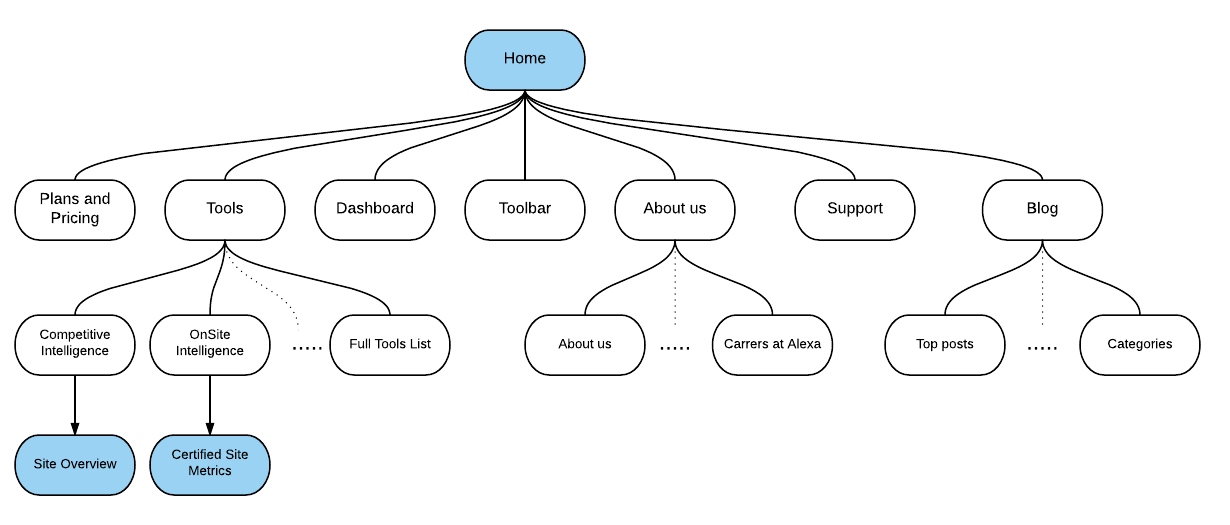
\includegraphics[scale=0.65,keepaspectratio]{{analisi/img/alexa_tree}.png}
    \caption{Struttura ad albero di alexa.com\protect\footnotemark}
    \end{figure}
    \FloatBarrier
Dal menù di navigazione il sito sembra avere un solo livello di profondità ma, analizzando attentamente ogni sezione, si nota come alcune di esse (i.e. About us) presentino una colonna a sinistra con delle voci indicanti altre sezioni. In
generale il sito risulta avere una profondità massima di livello 3.\\
Screenshot disponibile al path : \textit{Figure/2/sez0.png} \\ 
Altre sezioni sono implicitamente composte da sottosezioni presentate disponendo 
tutte le informazioni verticalmente nella 
pagina (come spiegato in \ref{scrolling}) e permettendo l'accesso ad
altre sottosezioni attraverso dei pulsanti disseminati nella pagina stessa. La 
scelta dei pulsanti risulta poco intuitiva per l'utente anche se 
usabile: i pulsanti sono di una grandezza proporzionale alla loro 
importanza (conseguenza della legge di Fitts) e risultano avere un buon 
contrasto rispetto allo sfondo oltre ad essere evidenziati nel momento in cui
vengono selezionati.
    \begin{figure}[ht]
    \centering
    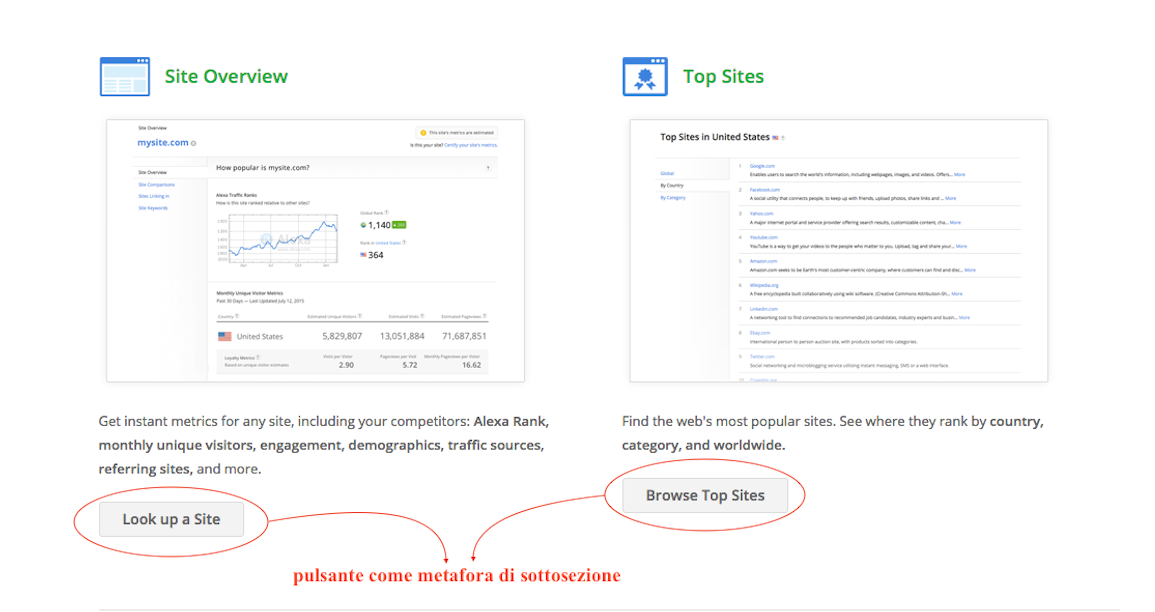
\includegraphics[scale=0.40,keepaspectratio]{{figure/2/sez1_particolare}.png}
    \caption{Pulsante come metafora di sezione di terzo livello}
    \end{figure}
    \FloatBarrier
Una nota negativa è data dalla sezione \textit{Support} 
che stravolge il layout standard eliminando totalmente il menù di navigazione e
presentando un'interfaccia che sembra essere totalmente estranea al sito, l'unico
modo per ritornare alla navigazione è cliccare sull'icona dell'azienda in alto
a sinistra che riporta alla homepage. \\
Screenshot disponibile al path : \textit{figure/2/sez2.png} \\ 
In conclusione la struttura non risulta molto chiara, anche se suddisiva in sezioni
pertinenti non aiuta l'utente ad orientarsi agevolmente all'interno del sito. \\
Risultato : \textit{5}
\footnotetext{evidenziate le sezioni analizzate in questo documento}

  \subsection{Sitemap}


\section{Homepage - assi informativi}
L’homepage rappresenta la vetrina del sito, è la sezione in cui l'utente 
decide se visitare o meno il sito web. 
Al fine di convincere l'utente è necessario fornire le informazioni 
necessarie a soddisfare le \quotes{6W}, ovvero una serie di domande
che l'utente si pone quando approda alla homepage di un 
qualsiasi sito web.
    \begin{figure}[ht]
    \centering
    
\includegraphics[scale=0.25,keepaspectratio]{{figure/3/home}.png}
    \caption{Homepage di alexa.com}
    \end{figure}
    \FloatBarrier 
  \subsection{Where}
\begin{center}

\textit{A che tipo di sito sono arrivato?}

Nella homepage del sito compare, in font sans serif di dimensione
più grande risepetto al resto del testo presente nella pagina, il motto: \\
\quotes{Your complete web analytics toolkit} \\
Grazie a questa informazione l'utente sa di trovarsi in un sito che offre
strumenti di ricerca per il web.

\end{center}
  \subsection{Who}\label{who}
\begin{center}

\textit{Chi rappresenta il sito?}


\end{center}
\begin{flushleft}
Il logo dell'azienda, il nome, e l'indicazione di appartenenza ad Amazon 
dicono chi rappresenta il sito. Importante notare come queste 
informazioni siano poste in una zona \quotes{calda} della pagina: risultano 
nell'angolo in alto a sinistra della forma ad \quotes{F} evidenziata 
dalle analisi di eyetracking. Per avere informazioni più specifiche sull'asse \textit{Who}
è necessario selezionare la sezione About nel menù di navigazione. \\
In generale l'asse \textit{Who} risulta soddisfatto. \\
Risultato : \textbf{8}
\end{flushleft}
  \subsection{Why}\label{why}
\begin{center}

\textit{Quali benefici offre il sito e quali sono le motivazioni per visitarlo?}

\end{center}
\begin{flushleft}
Come blurb al motto presente in Homepage viene spiegato quali benefici il sito 
possa offrire: \\
\quotes{an invaluable source for competitive intelligence and strategic insight}
\\
Per rendere più \quotes{umano} l'asse \quotes{Why}, e quindi convincere l'utente,
viene messo come sfondo della Homepage un CEO sorridente che utilizza i servizi di Alexa
per la sua azienda. A rimarcare ciò contribuisce la citazione sottostante al 
blurb appena descritto. Infine (sempre nella prima pagina)
vengono citate alcune aziende clienti di Alexa. Un'osservazione riguarda il contenuto
che, in questo caso, viene presentato in stile \quotes{slogan} e con poche informazioni
teniche e specifiche. Quest'ultima non è una buona prassi soprattutto perchè il target di utenza
per questa tipologia di siti è definito in partenza (vedi \ref{scopo}) e quindi
molto probabilmente gli utenti si aspettano delle informazioni più specifiche 
e potrebbero rimanere infastiditi dall'uso eccessivo di slogan. \\
Risultato : \textit{8.5}

\end{flushleft}
  \subsection{What}
\begin{center}

\textit{Cosa offre il sito?}

\end{center}
\begin{flushleft}
Questo asse non è subito visualizzabile in modo chiaro. Solo effetuando un 
primo scroll è possibile capire che strumenti di analisi web offre il sito.
Si sarebbe potuto evitare ciò riorganizzando meglio lo spazio della prima pagina senza scroll
o comunque sfruttando le colonne laterali che non vengono mai utilizzate nella homepage.
Le informazioni riguardanti l'asse \textit{What} non sono sempre organizzate in modo standard in 
tutte le pagine di scroll presenti in homepage:
\begin{itemize}
	\item la prima pagina di scroll utile le organizza a griglia;
	\item la seconda a lista;
	\item dalla terza pagina verticalmente (implica ulteriore scroll);
	\item dalla quinta ancora a lista fino all'ultima.
\end{itemize}
Queste diverse disposizioni
potrebbero affaticare l'utente nella navigazione della homepage. \\
Screenshot disponibile al path : \textit{figure/3/what0.png} \\
Un'altra osservazione
riguarda le immagini, in questo caso viene violata una convenzione web importante: 
\begin{center}
	\quotes{le immagini devono essere cliccabili}
\end{center}
Non tutte le immagini riguardanti l'asse \textit{What} sono cliccabili, l'unico modo 
di accedere alle funzionalità presentate è utilizzare il pulsante correlato 
che almeno risulta ben visibile e correttamente implementato (la zona cliccabile corrisponde a 
tutta la zona visibile). Le informazioni, anche se presentate in modo non ottimale,
risultano tuttavia esaustive.
    \begin{figure}[ht]
    \centering
    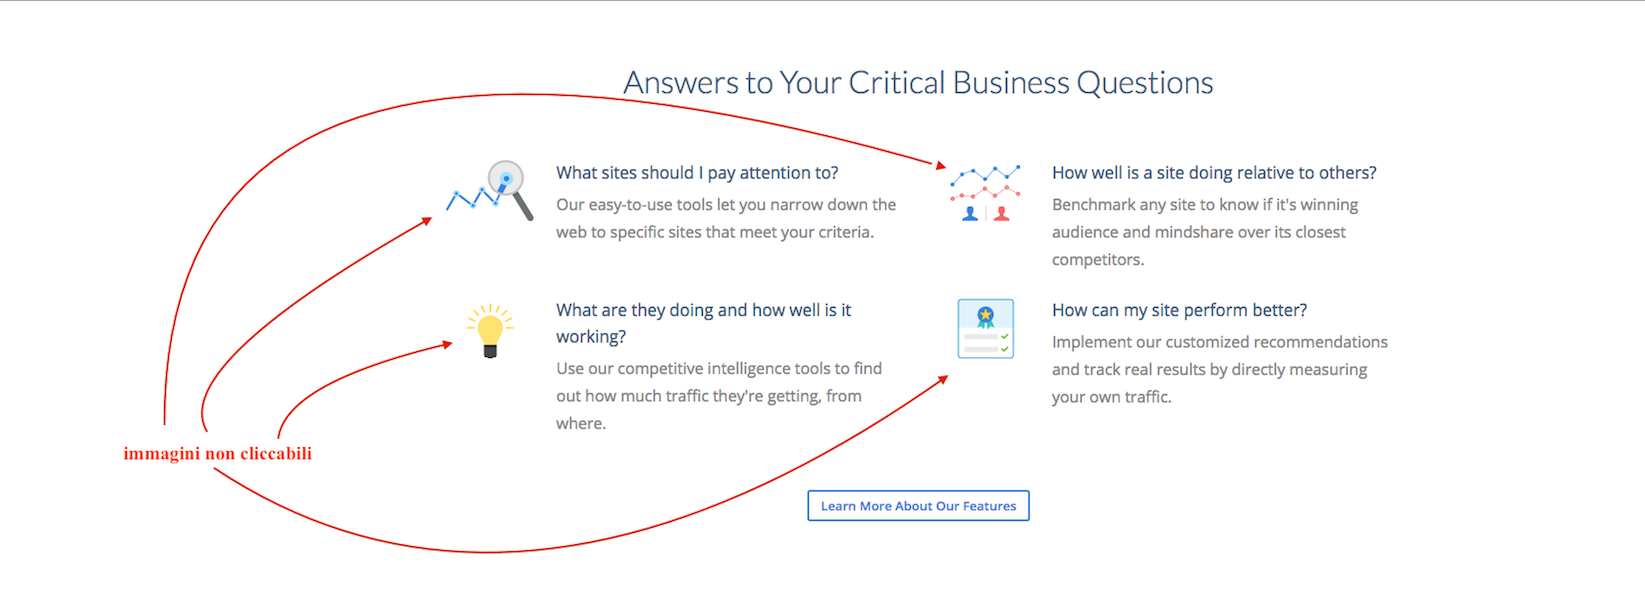
\includegraphics[scale=0.25,keepaspectratio]{{figure/3/what1}.png}
    \caption{Immagini non cliccabili}
    \end{figure}
    \FloatBarrier 
Risultato : \textbf{6}
\end{flushleft}
  \subsection{When}
\begin{center}

\textit{Quali sono le ultime novità? Quando è stato aggiornato l'ultima volta?}

\end{center}
  \subsection{How}\label{how}
\begin{center}

\textit{Come faccio ad arrivare alle sezioni principali?}

\end{center}
\begin{flushleft}
Il menù di navigazione non permette di muoversi agevolmente
in tutte le parti del sito in quanto molte sottosezioni sono \quotes{nascoste}
nell'utilizzo dei pulsanti (come spiegato in §\ref{sezioni}) compromettendo quasi totalmente la navigazione. \\
Risulta oneroso
consultare e cercare le informazioni di cui l'utente necessita.\\
Una possibile soluzione consiste in:
\begin{itemize}
	\item ridurre le molte pagine di scroll, presenti nella maggior parte
delle sezioni, e creare delle sezioni 
a profondità maggiore rendendo l'attuale menù a tendina (con due livelli
 di profondità sarebbe sufficiente);
\item dare al menù una posizione
fissa rispetto al browser in modo che, anche nel caso si utilizzasse lo scrolling
verticale, sia sempre possibile per l'utente avere le informazioni relative all'asse
\textit{How}.
\end{itemize}
    \begin{figure}[ht]
    \centering
    
\includegraphics[scale=0.38,keepaspectratio]{{figure/3/how0}.png}
    \caption{Homepage - Menù ad un solo livello}
    \end{figure}
    \FloatBarrier 
Risultato : \textit{3}
\end{flushleft}

\section{Pagine interne - caso d'uso}
  \subsection{Barra di ricerca}

  \subsubsection{Presentazione dei risultati di ricerca}
Mi riferisco alla presentazione dei risultati della funzionalità di ricerca
\quotes{Browser Top Sites}; la presentazione dei risultati del Box Testuale
discusso in precedenza è analoga a quella descritta in \ref{overview}.
\begin{figure}[ht]
\centering
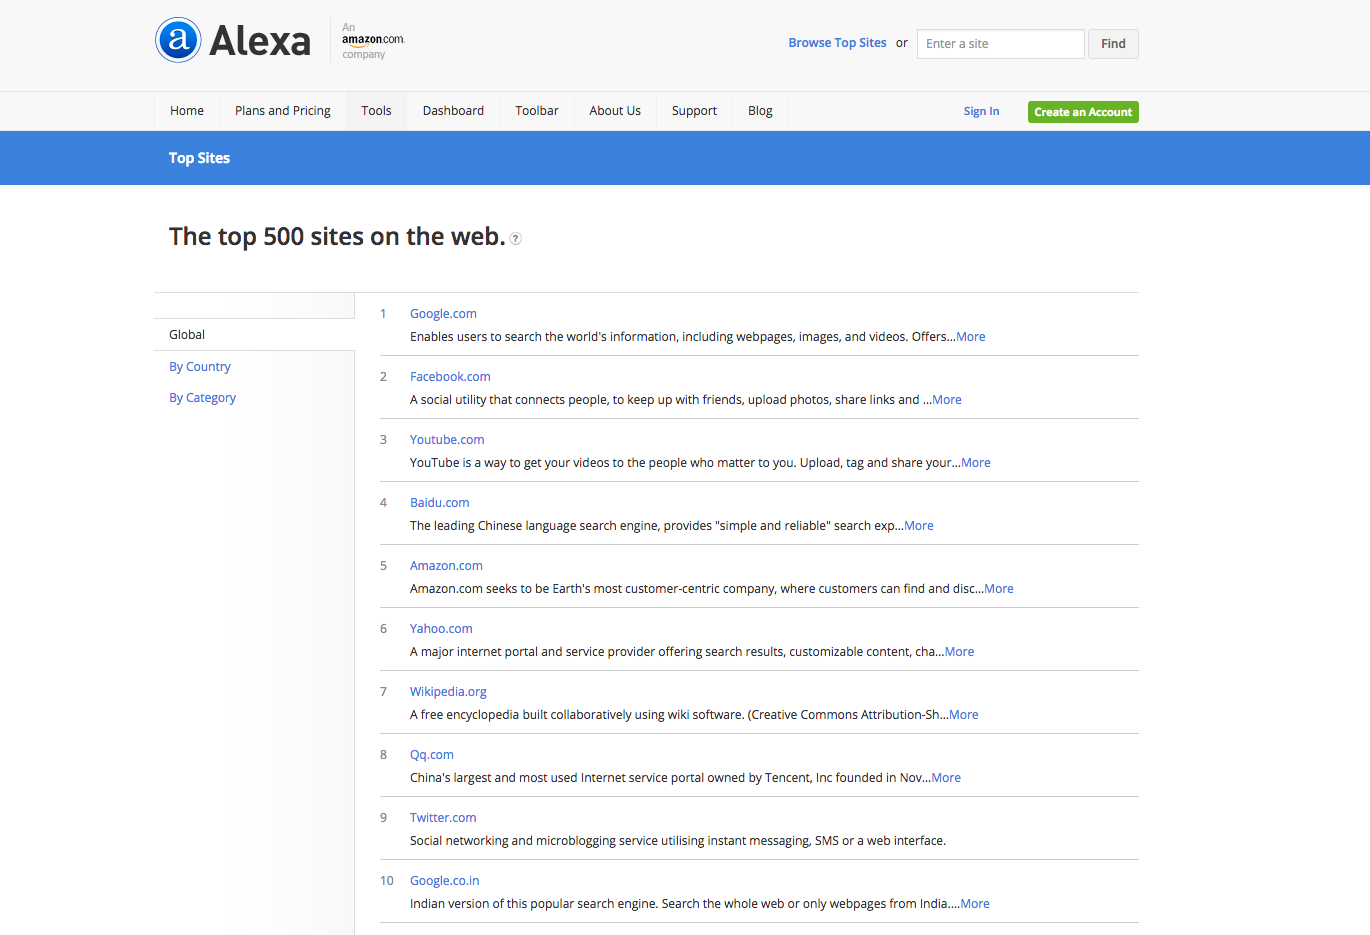
\includegraphics[scale=0.35,keepaspectratio]{{figure/4/searchResult0}.png}
\caption{Risultati di ricerca - Top Sites}
\end{figure}
\FloatBarrier
Ottima la presentazione dei risultati di ricerca: viene utilizzata una lista
numerata con un titolo ed una breve descrizione che si può facilmente espandere,
sulla colonna di sinistra sono indicati i filtri da utilizzare per visualizzare
i risultati. Nel bottom della pagina si possono selezionare i risultati
successivi alla prima pagina.\\
Risultato : \textbf{10}


\section{Valutazione}
Nel presente documento:
\begin{itemize}
	\item per ogni sottosezione di terzo livello (i.e. 2.2.1) 
	è stata data una valutazione in una scala da 0 (inclassificabile) a 10 (ottimo);
	\item per ogni sottosezione di secondo livello (i.e. 2.1) è stata calcolata
	la media aritmetica dei risultati ottenuti dalle relative sottosezioni di livello superiore a 3
	(come si può notare dalle voci presenti in tabella);
	\item la valutazione finale è composta dalla media pesata 
	(secondo importanza) dei risultati ottenuti dalle sottosezioni di secondo 
	livello.
\end{itemize}

\begin{longtable}{| p{5cm} | p{4cm} | l |}

\hline
\hline
\textbf{Aspetto} & \textbf{Valutazione} & \textbf{Peso} \\ 
\hline
\hline

\nameref{sezioni} & $4.5$ & $0.1$ \\%4.5
\hline
\nameref{general} & $6.63$ & $0.1$ \\%(9.8+6+9+0+5+10)/6 = 6.63
\hline
\nameref{where} & $8$ & $0.09$ \\%8
\hline
\nameref{who} & $8$ & $0.09$ \\%8
\hline
\nameref{why} & $8$ & $0.09$ \\%8
\hline
\nameref{what} & $6$ & $0.09$ \\%6
\hline
\nameref{when} & $5$ & $0.09$ \\%5
\hline
\nameref{how} & $3$ & $0.09$ \\%3
\hline
\nameref{usecase} & $8.65$ & $0.11$ \\%(7.5+9.8)/2 = 8.65
\hline
\nameref{searchfun} & $8.75$ & $0.07$ \\%(7.5+10)/2 = 8.75
\hline
\nameref{contenuto} &  $8$ & $0.08$ \\%(8.5+5.5+10)/3 = 8
\hline
\hline
\textbf{Totale} & \textbf{Valutazione$*$Peso} & \textbf{6.12} \\%((0.45+0.663+0.72+0.72+0.72+0.54+0.45+0.27+0.95+0.61+0.64)*10)/11
\hline
\hline
%
% 4.5*0.1
% 6.63*0.1
% 8*0.09
% 8*0.09
% 8*0.09
% 6*0.09
% 5*0.09
% 3*0.09
% 8.65*0.11
% 8.75*0.07
% 8*0.08
%
\end{longtable}

\appendix                               
\section{Lista delle figure}\label{figlist}

\begin{longtable}{| p{4.15cm} | p{5cm} | p{6.5cm} |}

\hline
\hline
\textbf{Figura} & \textbf{Path} & \textbf{URL} \\ 
\hline
\hline

\textit{404.png} & figure/2/404.png & \url{http://www.alexa.com/lukeskywlk} \\
\hline
\textit{sez0.png} & figure/2/sez0.png & \url{http://www.alexa.com/about} \\
\hline
\textit{sez1\_particolare.png} & figure/2/sez1\_particolare.png & \url{http://www.alexa.com/tools#competitive-intelligence} \\
\hline
\textit{sez2.png} & figure/2/sez2.png & \url{https://support.alexa.com/hc/en-us} \\
\hline
\textit{home0.png} & figure/3/home0.png & \url{http://www.alexa.com/} \\
\hline
\textit{how0.png} & figure/3/how0.png & \url{http://www.alexa.com/} \\
\hline
\textit{what0.png} & figure/3/what0.png & \url{http://www.alexa.com/} \\
\hline
\textit{what1.png} & figure/3/what1.png & \url{http://www.alexa.com/} \\
\hline
\textit{when0.png} & figure/3/when0.png & \url{http://www.alexa.com/} \\
\hline
\textit{where0.png} & figure/3/where0.png & \url{http://www.alexa.com/} \\
\hline
\textit{advertising0.png} &  figure/4/advertising0.png & \url{http://www.alexa.com/} \\
\hline
\textit{blurb0.png} & figure/4/blurb0.png & \url{http://www.alexa.com/} \\
\hline
\textit{images0.png} & figure/4/images0.png & \url{http://www.alexa.com/tools#competitive-intelligence} \\
\hline
\textit{searchBox0.png} & figure/4/searchBox0.png & \url{http://www.alexa.com/tools} \\
\hline
\textit{searchResult0.png} & figure/4/searchResult0.png & \url{http://www.alexa.com/topsites} \\
\hline
\textit{siteMetrics0.png} & figure/4/siteMetrics0.png & \url{http://www.alexa.com/tools#on-site-intelligence} \\
\hline
\textit{SiteOverviewSearch0.png} & figure/4/SiteOverviewSearch0.png & \url{http://www.alexa.com/tools#on-site-intelligence} \\
\hline
\textit{SiteOverviewSearch1.png} & figure/4/SiteOverviewSearch1.png & \url{http://www.alexa.com/siteinfo/baidu.com} \\
\hline
\textit{SiteOverviewSearch2.png} & figure/4/SiteOverviewSearch2.png & \url{http://www.alexa.com/siteinfo/baidu.com} \\
\hline
\textit{SiteOverviewSearch3.png} & figure/4/SiteOverviewSearch3.png & \url{http://www.alexa.com/siteinfo/baidu.com} \\
\hline
\textit{SiteOverviewSearch4.png} & figure/4/SiteOverviewSearch4.png & \url{http://www.alexa.com/siteinfo/baidu.com} \\
\hline
\hline
\end{longtable}

\end{document}
